\documentclass[11pt, twocolumn]{article}
\usepackage{graphicx, cite, verbatim, color, amsmath, amssymb}
\usepackage{listings}
\usepackage{hyperref}
\usepackage{fancyhdr}
\usepackage[compact]{titlesec}


%\setlength{\headheight}{0in}
\setlength{\headsep}{0.25in}
\setlength{\topmargin}{-0.25in}
\setlength{\textheight}{8.8in}
\setlength{\textwidth}{6.8in}
\setlength{\oddsidemargin}{-.15in}
\setlength{\evensidemargin}{-.15in}
\setlength{\unitlength}{1in}


% useful shortcuts/macros
\newcommand{\be}{\begin{eqnarray}}
\newcommand{\ee}{\end{eqnarray}}
\newcommand{\ben}{\begin{eqnarray*}}
\newcommand{\een}{\end{eqnarray*}}
\newcommand{\mbf}{\mathbf}
\newcommand{\mbfv}[1]{\vec{\mathbf{#1}}}
\newcommand{\sbf}[1]{\boldsymbol{#1}}
\newcommand{\half}{\frac{1}{2}}
\newcommand{\pp}[2]{\frac{\partial #1}{\partial #2}}
\newcommand{\dd}[2]{\frac{d #1}{d #2}}


% abstract formatting
\RequirePackage[style]{abstract}
\renewcommand{\abstitlestyle}[1]{}
\renewcommand{\abstracttextfont}{\bfseries\normalsize}
\setlength{\absleftindent}{0in}
\setlength{\absrightindent}{0in}

% caption formatting
\RequirePackage[tableposition=top]{caption}
\captionsetup*{font=bf}

% code listing formatting
\definecolor{commentgreen}{RGB}{14,120,0}
\lstset{
  numbers=none, 
  basicstyle=\scriptsize, 
  commentstyle=\color{commentgreen},
  keywordstyle=\bf\color{blue},
  language=python, 
  frame=shadowbox,
  rulesepcolor=\color{black},
  flexiblecolumns=true,
  extendedchars=false,
  showstringspaces=false,
  keepspaces=true
}

% packed itemize
\newenvironment{itemizePacked}{
\begin{itemize}
  \setlength{\itemsep}{0pt}
  \setlength{\parskip}{0pt}
  \setlength{\parsep}{0pt}
}{\end{itemize}}

% packed enumerate
\newenvironment{enumeratePacked}{
\begin{enumerate}
  \setlength{\itemsep}{-1pt}
  \setlength{\parskip}{0pt}
  \setlength{\parsep}{0pt}
}{\end{enumerate}}


% no indent
\setlength{\parindent}{0pt}

% column separation
\setlength{\columnsep}{3ex}

% header
\fancyhead[L]{
\large \sc
AE 623 Winter 2026 \quad Group Name \quad Project 1
}
\renewcommand{\headrulewidth}{1pt}
\pagestyle{fancy}

% section spacing
\titlespacing{\section}{0pt}{12pt}{4pt}
\titlespacing{\subsection}{0pt}{8pt}{2pt}



%******************************************************************************
\begin{document}


\title{\vspace{-5ex} \bf AE 623 Project Report Template}

\author{First Author, Second Author, Third Author, Fourth Author, and Fifth Author\\
\emph{Group Name}}

\maketitle

\begin{abstract}
This template presents the format of a technical report for AE 623.
The abstract should summarize the problem, approach, and key results.
It should be one paragraph.
\end{abstract}


%==============================================================================
\section{Introduction}

Technical reports must not exceed 10 pages in length, using the font
size and margins specified in this template.  Figures, references,
appendices, code snippets, and effort breakdown all count towards
the 10 page limit.  You are encouraged to use Latex and this template.
You are allowed to use other typesetting tools, e.g. Word, but you
must emulate this template as closely as possible.

The introduction should state the problem, any relevant literature
background, and a brief overview of the solution approach.  Citations
should be hyperlinked and referred to by number
only~\cite{Reed_Hill_1973}, unless starting a sentence.
Ref.~\cite{Reed_Hill_1973} presents one of the first discontinuous
Galerkin implementations.


%==============================================================================
\section{Methods}

Describe the methods you use to solve the given tasks, and include key
derivations, or outlines thereof, as needed.  Be complete, but avoid
repetition and lengthy derivations -- you do not need to demonstrate
your ability to perform routine mathematical tasks, such as applying
the chain rule, or solving/manipulating algebraic equations.  Do not
include a nomenclature, and instead define the symbols as you use
them.



%------------------------------------------------------------------------------
\subsection{Governing Equations}

We consider the Euler equations of gas dynamics, 
%
\be
\label{e:Euler}
\pp{\mbf{u}}{t} + \nabla \cdot \mbfv{F} = \mbf{0},
\ee
%
where in two dimensions, the conservative state is $\mbf{u} = [\rho,
  \rho u, \rho v, \rho E]^T$, and $\mbfv{F} = \mbf{F} \hat{x} +
\mbf{G} \hat{y}$ is the flux vector. While Eqn.~\ref{e:Euler} is
unsteady, in this project we are only concerned with the steady-state
solution.



%------------------------------------------------------------------------------
\subsection{Algorithms and Code }

Discuss your high-level code structure, including memory layout, key
loops, initialization, user interface, run scripts, post-processing,
and any trade-offs between storage and computation.  You can present
algorithms, or portions thereof, in pseudocode.  Small code snippets,
such as the one given in Listing~\ref{l:hello}, may be useful, but do
not include large code sections.  Make sure your code, which you need
to include in the \texttt{.zip} archive, is neat and commented.
Describe any tests you performed on your code.


\lstinputlisting[
  linerange=3-12,
  linewidth=1.0\linewidth,
  xleftmargin=0.0\linewidth,
  caption={Sample code snippet},
  label=l:hello,
]{hello.py}



%==============================================================================
\section{Results}

Present the results requested in the project statement, broken down by
task or by other criteria, as you deem appropriate.  Ensure that
figures are of high resolution and that plots are labelled and
captioned.  Include a discussion of the results.

%------------------------------------------------------------------------------
\subsection{Task 1}

Figure~\ref{f:mach} shows the computational mesh and Mach number
contours for a 5th-order simulation of inviscid flow over a
multi-element airfoil.

\begin{figure}[htpb!]
  \centering
  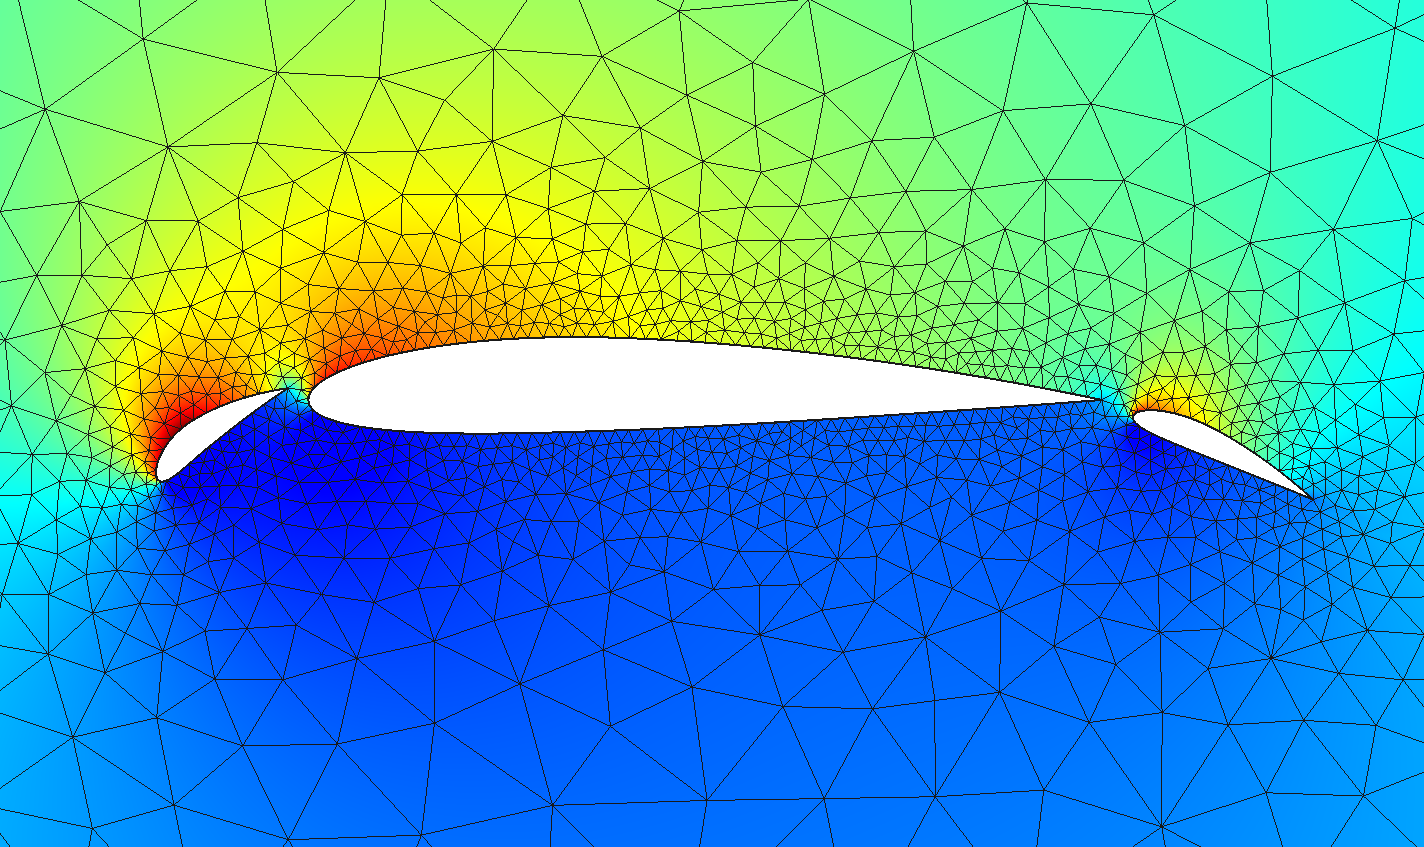
\includegraphics[width=1.0\columnwidth]{mach.png}
  \caption{\label{f:mach} Mach contours (0-0.7) for a multi-element
    airfoil at free-stream Mach number 0.2 and angle of attack $\alpha
    = 10^{\circ}$. }
\end{figure}


%------------------------------------------------------------------------------
\subsection{Task 2}

Table ~\ref{t:table} presents a sample table.


\begin{table}[htbp!]
  \centering
  \caption{\label{t:table} Lift coefficient data.}
  \begin{tabular}{cccc}
    %\hline
    Mesh & \# cells & order & $c_{\ell}$ \\
    \hline \hline \\ [-2ex]
    coarse & 2000 & 1 & 0.53 \\
    medium & 8000 & 1 & 0.57 \\
    medium & 8000 & 2 & 0.61
  \end{tabular}
\end{table}



%==============================================================================
\section{Conclusions}

Summarize the problem, tasks, results, and draw take-away conclusions.


%==============================================================================
\section{Effort Breakdown}

Write a few sentences explaining how each group member contributed to
the project, and include Table~\ref{t:effort} -- use initials for the
column headers, and make sure each row adds up to 100\%.  Development
refers to research, analysis, derivations, and code planning.  Coding
is writing of the computer code.  Examples of managing are
coordinating meeting times, assigning tasks, setting up shared
repositories or documents, etc.  Report refers to writing and
formatting the report.  The effort breakdown does not need to be
uniform, and grades will only be affected in cases of severe and
consistent disparities.

\begin{table}[htbp!]
  \centering
  \caption{\label{t:effort} Effort percentages.}
  \begin{tabular}{lrrrrr}
    %\hline
     & 1A & 2A & 3A & 4A & 5A  \\
    \hline \hline \\ [-2ex]
    development & 50 & 10 & 10 & 15 & 15 \\
    coding &  20 & 35 & 15 & 15 & 15 \\
    managing & 10 & 10 & 10 & 60 & 10 \\
    report & 20 & 20 & 20 & 20 & 20
  \end{tabular}
\end{table}





%==============================================================================
% References
\bibliographystyle{plain}
\small
\bibliography{main}


\end{document}
